%% !TEX program = xelatex
%% !BIB program = bibtex
\documentclass[10pt,aspectratio=169]{beamer}  % present

\mode<presentation>
{
    \usetheme{default}   % or try Boadilla, boxes, Singapore, Darmstadt, Madrid, Warsaw, ...
    \usecolortheme{default} % or try albatross, beaver, crane, ...

    \usefonttheme{structurebold}  % or try serif, , ...
    \setbeamertemplate{navigation symbols}{}
    \setbeamertemplate{caption}[numbered]
    \definecolor{MyColor}{rgb}{0,0.3,0.65}
    \definecolor{MyColorLight}{rgb}{0,0.7,0.95}
    \definecolor{MyGreenColor}{rgb}{0,0.6,0}
    \definecolor{MyRedColor}{rgb}{0.8,0,0}
    \setbeamercolor{structure}{fg=MyColor}
}

%% Packages
\usepackage[round]{natbib}
%\usepackage{authblk}
\usepackage{amsfonts,amsmath,amssymb,mathtools,marvosym,amsthm,ulem,cancel}
%\usepackage{enumerate}
\usepackage{graphicx,float,tcolorbox}
\hypersetup{colorlinks,linkcolor=MyColor,citecolor=MyColor,urlcolor=black,breaklinks=true}
% \usepackage{fontspec}
% \usepackage{tikz}

%% Print author name, short title, date and slide number at the bottom of the page
% \setbeamercolor{author in head/foot}{fg=MyColor, bg=MyColorLight}
\makeatletter
\setbeamertemplate{footline}
{
    \leavevmode%
    \hbox{%
        \begin{beamercolorbox}[wd=.333333\paperwidth,ht=2.25ex,dp=1ex,center]{author in head/foot}%
            \usebeamerfont{author in head/foot}\insertshortauthor
        \end{beamercolorbox}%
        \begin{beamercolorbox}[wd=.333333\paperwidth,ht=2.25ex,dp=1ex,center]{title in head/foot}%
            \usebeamerfont{title in head/foot}\insertshorttitle
        \end{beamercolorbox}%
        \begin{beamercolorbox}[wd=.333333\paperwidth,ht=2.25ex,dp=1ex,right]{date in head/foot}%
            \usebeamerfont{date in head/foot}\insertshortdate{}\hspace*{2em}
            \insertframenumber{} / \inserttotalframenumber\hspace*{2ex}
        \end{beamercolorbox}%
    }%
    \vskip0pt%
}
\makeatother

% \setmainfont{Ubuntu}
% \setmainfont{DejaVu Serif}
% \setsansfont{Segoe UI}
% \setsansfont{EB Garamond}
% \setsansfont{Tahoma}
% \setsansfont{Roboto}
% \setsansfont{Open Sans}
% \setsansfont{Georgia}
% \setsansfont{SF Pro Display}
% \setsansfont{Lato}
% \setmonofont{Monospaced}


%\setlength{\parindent}{0.5cm}
\setlength{\parskip}{0.3cm}

\renewcommand{\baselinestretch}{1.0}
\renewcommand{\arraystretch}{1.2}

\newtheorem{proposition}{Proposition}

% ------------------------------------------------------------------------------

%% Description
\author[Narek Ohanyan]{Narek Ohanyan}
\title[Dynamic Nature of Relationships]{Lecture 1. Dynamic Nature of Relationships}
\institute[AUA]{American University of Armenia}
\date{\today}

% ------------------------------------------------------------------------------

%% Add table of contents before every subsection
\AtBeginSection[]
{
    \begin{frame}{Outline}
        \tableofcontents[currentsection]
    \end{frame}
}

% ==============================================================================

\begin{document}

\begin{frame}
    \titlepage
\end{frame}

% ------------------------------------------------------------------------------

\section{Time Series Data}

\begin{frame}{Nature of time series data}

    \bigskip

    The nature of the data available has an important bearing on the appropriate choice of an econometric model.

    Two features of time-series data to consider:
    \begin{enumerate}\itemsep=1em
        \item Time-series observations on a given economic unit, observed over a number of time periods, are likely to be correlated
        \item Time-series data have a natural ordering according to time
    \end{enumerate}

\end{frame}

% ------------------------------------------------------------------------------

\begin{frame}{Stationary and nonstationary time series}

    \bigskip

    A time series is said to be \textbf{stationary} if its mean and variance are constant over time.

    \medskip
    A time series is said to be \textbf{nonstationary} if its mean and variance are not constant over time.

    \medskip
    In other words, a stationary variable is one that is not trending, and nor wandering aimlessly without returning to its mean.

    \medskip
    Stationarity is an important property because many time series models are based on the assumption that the data are stationary.

\end{frame}

% ------------------------------------------------------------------------------

\begin{frame}{Different types of time series}

    \bigskip
    \begin{figure}[H]
        \centering
        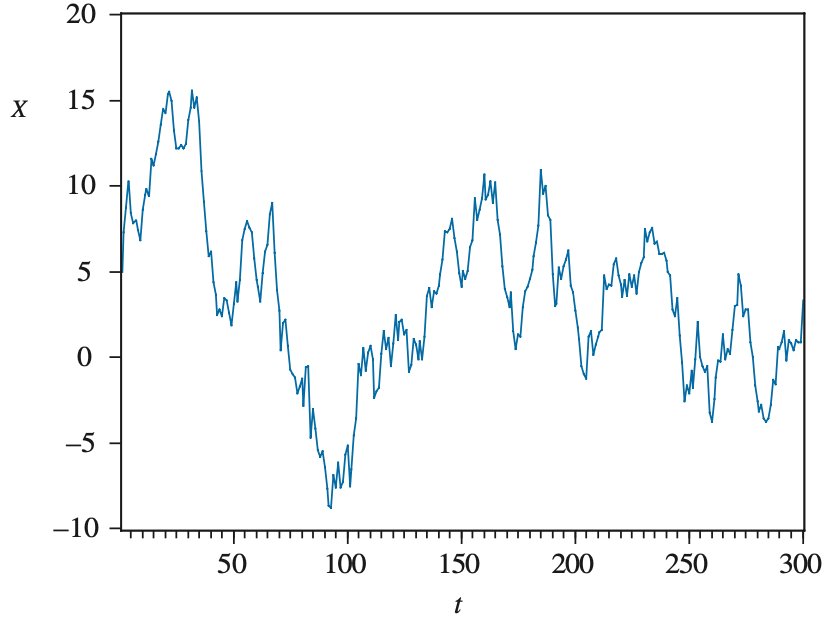
\includegraphics[height=0.4\textwidth]{./fig/random-walk.png}
    \end{figure}

\end{frame}

% ------------------------------------------------------------------------------

\begin{frame}{Different types of time series}

    \bigskip
    \begin{figure}[H]
        \centering
        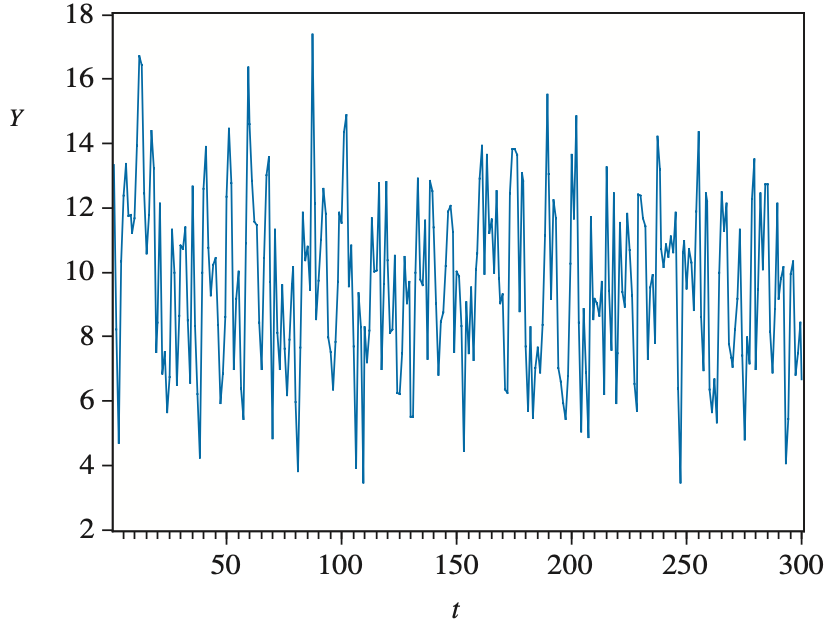
\includegraphics[height=0.4\textwidth]{./fig/autoregressive.png}
    \end{figure}

\end{frame}

% ------------------------------------------------------------------------------

\begin{frame}{Different types of time series}

    \bigskip
    \begin{figure}[H]
        \centering
        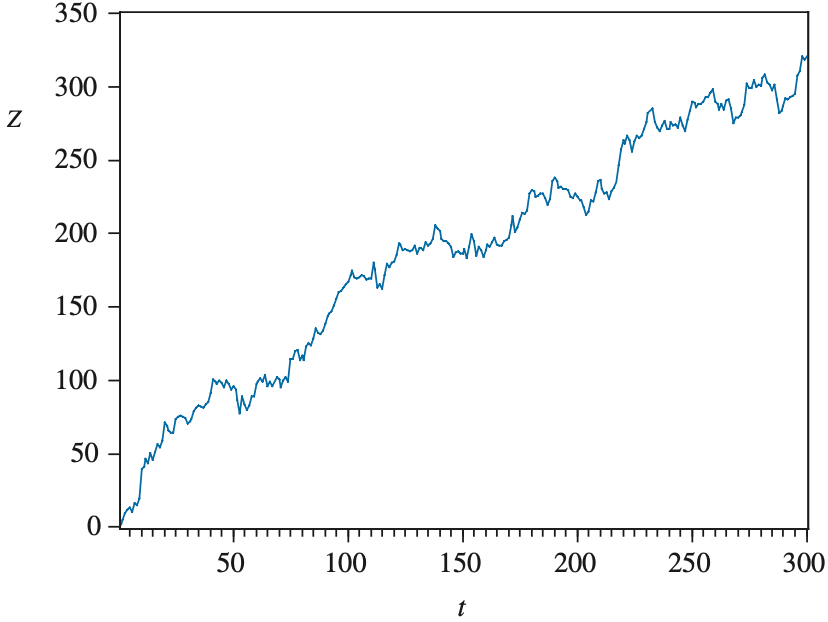
\includegraphics[height=0.4\textwidth]{./fig/random-walk-with-trend.png}
    \end{figure}

\end{frame}

% ==============================================================================

\section{Dynamic Relationships}

% ------------------------------------------------------------------------------

\begin{frame}{Dynamic relationships}

    \bigskip
    In many economic applications, the relationship between two variables is \textbf{dynamic}.

    \medskip
    That is, the change in a variable may have an impact on itself, or other variables, in one or more future time periods
    \begin{figure}[H]
        \centering
        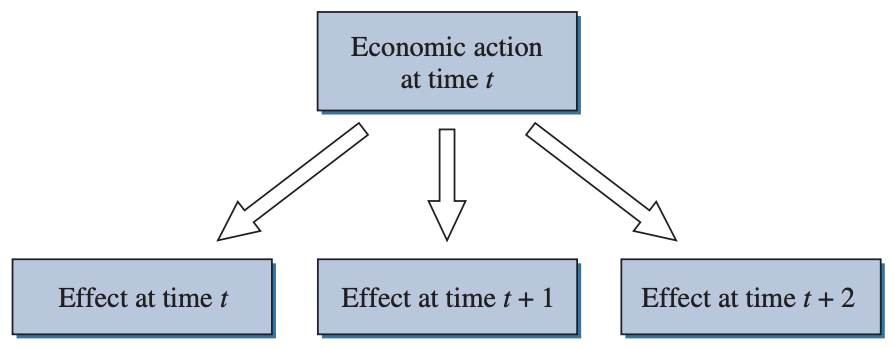
\includegraphics[height=0.2\textwidth]{./fig/dynamic-effects.png}
    \end{figure}

\end{frame}

% ------------------------------------------------------------------------------

\begin{frame}{Modelling dynamic relationships}

    \bigskip

    There may be three different types of dynamic relationships:
    \begin{enumerate}
        \item The dependent variable $ y $ may be a function of current and past values of an explanatory variable $ x $
        \begin{align*}
            y_{t} = f(x_{t}, x_{t-1}, x_{t-2}) + e_{t}
        \end{align*}
        \item The dependent variable $ y $ may be a function of its own past values
        \begin{align*}
            y_{t} = f(y_{t-1}, x_{t}) + e_{t}
        \end{align*}
        \item The error term $ u $ may be a function of its own past values
        \begin{align*}
            & y_{t} = f(x_{t}) + e_{t} \\
            & e_{t} = g(e_{t-1}) + \varepsilon_{t}
        \end{align*}

    \end{enumerate}

\end{frame}

% ------------------------------------------------------------------------------

\begin{frame}{Distributed lag models}

    \bigskip

    The first type of dynamic relationship is called a \textbf{distributed lag model}.

    \medskip
    Suppose that the variable $ y $ depends on current and past values of variable $ x $, up to $ q $ periods into the past
    \begin{align*}
        y_{t} = \alpha + \beta_{0} x_{t} + \beta_{1} x_{t-1} + \beta_{2} x_{t-2} + \cdots + \beta_{q} x_{t-q} + e_{t}
    \end{align*}

    \medskip
    \begin{itemize}
        \item The coefficient $ \beta_{0} $ is called the \textit{impact} multiplier.
        \item The coefficients $ \beta_{s} $ are called the s-period \textit{delay} multipliers.
    \end{itemize}

\end{frame}

% ------------------------------------------------------------------------------

\begin{frame}{Dynamic effects in distributed lag models}

    \bigskip

    Recall that the distributed lag model is
    \begin{align*}
        y_{t} = \alpha + \beta_{0} x_{t} + \beta_{1} x_{t-1} + \beta_{2} x_{t-2} + \cdots + \beta_{q} x_{t-q} + e_{t}
    \end{align*}

    Assume $ x_{t} $ is increased by one unit and then maintained at its new level in subsequent periods.
    \begin{itemize}
        \item The immediate impact at $ t $ will be $ \beta_{0} $
        \item The effect in period $ t + 1 $ will be $ \beta_{0} + \beta_{1} $
        \item The effect in period $ t + 2 $ will be $ \beta_{0} + \beta_{1} + \beta_{2} $ and so on
    \end{itemize}

    Th cumulative effect of a change in $ x_{t} $ on $ y_{t} $ is called \textbf{interim multiplier}.

    The \textbf{total multiplier} is the final effect on $ y $ of the sustained increase after $ q $ or more periods have elapsed.

\end{frame}

% ------------------------------------------------------------------------------

\begin{frame}{Autorergressive models}

    \bigskip

    The second type of dynamic relationship is called an \textbf{autoregressive model}.

    \medskip
    Suppose that the variable $ y $ depends on its own past values, up to $ p $ periods into the past
    \begin{align*}
        y_{t} = \alpha + \phi_{1} y_{t-1} + \phi_{2} y_{t-2} + \cdots + \phi_{p} y_{t-p} + e_{t}
    \end{align*}

    The model is called an autoregressive model of order $ p $, or an $ AR(p) $ model.

\end{frame}

% ------------------------------------------------------------------------------

\begin{frame}{Dynamic effects in autoregressive models}

    \bigskip

    Recall that the autoregressive model is
    \begin{align*}
        y_{t} = \alpha + \phi_{1} y_{t-1} + \phi_{2} y_{t-2} + \cdots + \phi_{p} y_{t-p} + e_{t}
    \end{align*}

    Suppose that $ y_{t} $ is increased by one unit and then maintained at its new level in subsequent periods.
    \begin{itemize}
        \item The effect in period $ t + 1 $ will be $ \phi_{1} $
        \item The effect in period $ t + 2 $ will be $ \phi_{1}^2 + \phi_{2} $
        \item The effect in period $ t + 3 $ will be $ \phi_{1}^3 + 2 \phi_{1}\phi_{2} + \phi_{3} $ and so on
    \end{itemize}

\end{frame}

% ------------------------------------------------------------------------------

\begin{frame}{Autorergressive distributed lag models}

    \bigskip

    We can combine the two types of dynamic relationships into a single model, called an \textbf{autoregressive distributed lag model}
    \begin{align*}
        y_{t} = \alpha + \phi_{1} y_{t-1} + \cdots + \phi_{p} y_{t-p} + \beta_{0} x_{t} + \beta_{1} x_{t-1} + \cdots + \beta_{q} x_{t-q} + e_{t}
    \end{align*}

    The model is called an autoregressive distributed lag model of order $ p $ and $ q $, or an $ ARDL(p, q) $ model.

\end{frame}

% ------------------------------------------------------------------------------

\begin{frame}{Models with autoregressive errors}

    \bigskip

    The third type of dynamic relationship is called a \textbf{model with autoregressive errors}.

    \medskip
    Suppose that the error term $ e_{t} $ depends on its own past value
    \begin{align*}
        y_{t} = \alpha + \beta_{0} x_{t} + e_{t} \\
        e_{t} = \rho e_{t-1} + \varepsilon_{t}
    \end{align*}

    Substituting the second equation into the first yields
    \begin{align*}
        y_{t} = \delta + \rho y_{t-1} + \beta_{0} x_{t} + \beta_{1} x_{t-1} + \varepsilon_{t}
    \end{align*}
    where $ \delta = \alpha \left( 1-\rho \right) $ and $ \beta_{1} = - \rho \beta_{0} $.

    Hence, the model with autoregressive errors is a special case of an $ ARDL(1, 1) $ model.

\end{frame}

% ==============================================================================

\section{Autoregressive and Moving Average Models}

% ------------------------------------------------------------------------------

\begin{frame}{White noise and IID processes}

    \bigskip
    The basic building block of time-series models is the \textit{white noise} process.

    \medskip
    A random variable $ e_{t} $ is called \textbf{white noise (WN)} if
    \begin{align*}
        & \mathrm{E}(e_{t}) = 0 \\
        & \mathrm{Var}(e_{t}) = \sigma^2 \\
        & \mathrm{Cov}(e_{t}, e_{t-s}) = 0 \quad \text{for all} \quad s \neq 0
    \end{align*}
    A random variable $ e_{t} $ is called \textbf{independent and identically distributed (IID)} if
    \begin{align*}
        & F \left( e_{t} \right) = F \left( e_{t-s} \right) \quad \text{for all} \quad s \\
        & e_{t} \: \perp \: e_{t-s} \quad \text{for all} \quad s \neq 0
    \end{align*}
    where $ F \left( e_{t} \right) $ is the cumulative distribution function of $ e_{t} $.

    \medskip
    An IID process is also a WN process.

\end{frame}

% ------------------------------------------------------------------------------

\begin{frame}{Serial correlation}

    \bigskip
    Autocorrelation, or serial correlation, is the correlation between a variable and its past or future values.

    \medskip
    The \textbf{autocovariance} of a variable $ x $ at lag $ k $ is defined as
    \begin{align*}
        \mathrm{Cov}(x_{t}, x_{t-k}) = \mathrm{E} \left[ (x_{t} - \mu_{x})(x_{t-k} - \mu_{x}) \right]
    \end{align*}

    Then, the \textbf{autocorrelation} coefficient of $ x $ at lag $ k $ is
    \begin{align*}
        \rho_{k} = \frac{\mathrm{Cov}(x_{t}, x_{t-k})}{\mathrm{Var}(x_{t})}
    \end{align*}

    \medskip
    The autocorrelation coefficients $ \rho_{k} $ take values between $ -1 $ and $ 1 $.

\end{frame}

% ------------------------------------------------------------------------------

\begin{frame}{AR(1) model}

    \bigskip
    The simplest autoregressive model is the $ AR(1) $ model
    \begin{align*}
        y_{t} = c + \phi y_{t-1} + e_{t} \qquad e_{t} \sim WN(0, \sigma^2)
    \end{align*}

    We assume that $ \left| \phi \right| < 1 $, so that the model is stationary.

    \medskip
    The mean and variance of $ y_{t} $ are
    \begin{align*}
        \mathrm{E}(y_{t}) = \frac{c}{1 - \phi} \qquad \mathrm{Var}(y_{t}) = \frac{\sigma^2}{1 - \phi^2}
    \end{align*}
    The autocovariance of $ y_{t} $ at lag $ k $ is
    \begin{align*}
        \mathrm{Cov}(y_{t}, y_{t-k}) = \phi^k \frac{\sigma^2}{1 - \phi^2}
    \end{align*}
    The autocorrelation of $ y_{t} $ at lag $ k $ is
    \begin{align*}
        \rho_{k} = \phi^k
    \end{align*}

\end{frame}

% ------------------------------------------------------------------------------

\begin{frame}{MA(1) model}

    \bigskip
    The simplest moving average model is the $ MA(1) $ model
    \begin{align*}
        y_{t} = c + e_{t} + \theta e_{t-1} \qquad e_{t} \sim WN(0, \sigma^2)
    \end{align*}

    \medskip
    The mean and variance of $ y_{t} $ are
    \begin{align*}
        \mathrm{E}(y_{t}) = c \qquad \mathrm{Var}(y_{t}) = \sigma^2 \left( 1 + \theta^2 \right)
    \end{align*}
    The autocovariance of $ y_{t} $ at lag $ k $ is
    \begin{align*}
        \mathrm{Cov}(y_{t}, y_{t-k}) = \theta \sigma^2 \quad \text{for} \quad k = 1 \quad \text{and} \quad \mathrm{Cov}(y_{t}, y_{t-k}) = 0 \quad \text{for} \quad k \geq 2
    \end{align*}
    The autocorrelation of $ y_{t} $ at lag $ k $ is
    \begin{align*}
        \rho_{k} = \frac{\theta}{1 + \theta^2} \quad \text{for} \quad k = 1 \quad \text{and} \quad \rho_{k} = 0 \quad \text{for} \quad k \geq 2
    \end{align*}

\end{frame}

% ------------------------------------------------------------------------------

\begin{frame}{Autocorrelation and partial autocorrelation}

    \bigskip
    \textbf{Autocorrelation}

    Recall that the \textit{autocorrelation} coefficient of $ y_{t} $ at lag $ k $ is the correlation between $ y_{t} $ and $ y_{t-k} $
    \begin{align*}
        \rho_{k} = \frac{\mathrm{Cov}(y_{t}, y_{t-k})}{\mathrm{Var}(y_{t})}
    \end{align*}

    \medskip
    \textbf{Partial autocorrelation}

    The \textit{partial autocorrelation} coefficient of $ y_{t} $ at lag $ k $ is the correlation between $ y_{t} $ and $ y_{t-k} $ after removing the effect of the intermediate lags $ y_{t-1}, y_{t-2}, \ldots, y_{t-k+1} $.

    \begin{align*}
        \phi_{k,k} = \frac{\mathrm{Cov}(y_{t}, y_{t-k} | y_{t-1}, \ldots, y_{t-k+1})}{\mathrm{Var}(y_{t} | y_{t-1}, \ldots, y_{t-k+1})}
    \end{align*}

\end{frame}

% ------------------------------------------------------------------------------

\begin{frame}{ACF and PACF plots}

    \bigskip
    Autocorrelation and partial autocorrelation functions plot the $ \rho_{k} $ and $ \phi_{k,k} $ against $ k $.

    \medskip
    For an $ AR(p) $ model
    \begin{itemize}
        \item The ACF plot will show gradual \textbf{decay} before and after lag $ p $,
        \item The PACF plot will show a sharp \textbf{cutoff} after lag $ p $.
    \end{itemize}

    For an $ MA(q) $ model
    \begin{itemize}
        \item The ACF plot will show a sharp \textbf{cutoff} after lag $ q $,
        \item The PACF plot will show gradual \textbf{decay} before and after lag $ q $.
    \end{itemize}

    \medskip
    Hence, ACF and PACF plots can be used to identify the \textbf{order} of an AR or MA model.

\end{frame}

% ==============================================================================

\section{Testing for Serial Correlation}

% ------------------------------------------------------------------------------

\begin{frame}{Estimation and testing for autocorrelation}

    \bigskip
    The sample autocorrelation coefficient of $ x $ at lag $ k $ is
    \begin{align*}
        \widehat{\rho}_{k} = \frac{\sum_{t=k+1}^{T} \left( x_{t} - \bar{x} \right) \left( x_{t-k} - \bar{x} \right)}{\sum_{t=1}^{T} \left( x_{t} - \bar{x} \right)^2}
    \end{align*}

    \medskip
    Since $ \rho_{k} = 0 $ means no autocorrelation, we are often interested in the following hypothesis $ \mathrm{H}_{0}: \rho_{k} = 0 $ versus $ \mathrm{H}_{1}: \rho_{k} \neq 0 $.

    \medskip
    The test statistic is
    \begin{align*}
            \sqrt{T} \widehat{\rho}_{k} \: \sim \: \mathcal{N}(0, 1)
    \end{align*}

    A sample autocorrelation function plot may also be used for visualizing and testing for autocorrelation.

\end{frame}

% ------------------------------------------------------------------------------

\begin{frame}{Sample autocorrelation function (ACF)}

    \bigskip

    A sample autocorrelation function (ACF) plot or \textbf{correlogram} is a plot of $ \widehat{\rho}_{k} $ against $ k $.

    \vspace{-0.3cm}
    \begin{figure}[H]
        \centering
        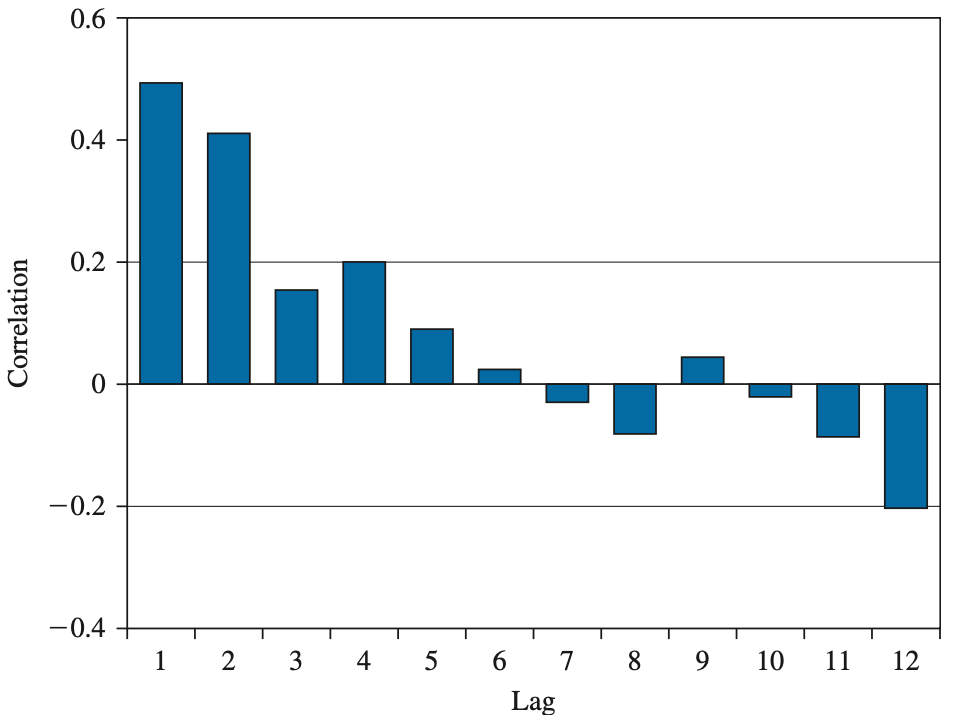
\includegraphics[height=0.35\textwidth]{./fig/correlogram.png}
    \end{figure}
    \vspace{-0.4cm}

    Confidence intervals of $ \pm 1.96/\sqrt{T} $ are also commonly plotted to help identify significant autocorrelation coefficients.

\end{frame}

% ==============================================================================

% % \begin{frame}<beamer:0>
% \begin{frame}[allowframebreaks]{Bibliography}

%     \bibliographystyle{apalike}
%     \bibliography{references}

% \end{frame}

% ==============================================================================

\end{document}
